\chapter{设计与实现}
\label{chap:design}


本章我们将介绍云搜索正确性的快速验证系统的整个系统构造。首先,我们会介绍该系统的整体框架,介绍它是有那些部分组成的,每个部分是什么功能的以及各个部分之间是怎么交互的。然后,我们会介绍整个系统里面一些重要的细节,比如为了提升整体效率而设计的一些方案,比如树状的证明结构。

\section{系统的整体架构}

我们使用了第\ref{chap:relatedwork}章介绍的验证机制来进行云搜索的正确性验证。按照该验证机制的特点,我们进行了有针对性的系统设计。该验证机制包含两个角色,数据拥有着(用户)和云服务商。对此,我们将系统划分为客户端和服务端。在云端,我们需要完成索引的查询以及搜索结果的生成等操作,我们按照功能进行了相应的模块划分。

在我们的系统里,每个模块都是一个可以单独启动的进程,模块之间使用HTTP协议进行交互。采用这样设计的原因主要是:1. 采用单独的进程可以让每个模块进行单独的部署,而不需要都部署到一台机器,这样使得系统有比较好的可扩展性,2. HTTP是一种使用得非常广泛也非常易于使用的协议,采用HTTP可以让我们的系统可以更加容易进行调试也方便了一些扩展模块的开发。

具体的,考虑到高可靠性,扩展性,高可维护性的要求,我们将系统分为了Index Generator, Search Client, Search Server, Query Node, Correctness Server, Integrity Server, Prime Manager这几个组成部分。我们会在后续的内容中对这几个组成部分分别进行介绍。

我们的系统采用了C++来进行实现,用到了很多boost库的内容,比如利用了其中的Asio来进行异步的HTTP请求。在高精度计算方面,我们采用了NTL这个C++库,并采用了GMP加速。

下面我们按照模块对云搜索正确性的快速验证系统进行介绍。

\myfig{framework.eps}{3.5in}{系统的整体框架 }{des:structure}{Structure of system}

\subsection{Index Generator}
Index Gnerator是一个单独的工具,它不需要和别的模块进行交互。它主要负责的对于一个文本的集合进行可验证索引的建立操作。我们采用了Indri Indexer\cite{Indri}来生成倒排索引。在生成了倒排索引之后,我们从中抽取出我们需要的内容,用来生成可验证索引。对于生成的可验证索引,我们以文件的形式存储到磁盘上。索引的数据比较大,为了减少单个文件的体积,同时也为了方便使用多模块处理,我们将索引数据使用一致性哈希的方式存储到多个文件中。生成的索引数据文件组织如下:
\begin{itemize}
\item \textbf{meta.txt} 存储索引数据的元信息,包括索引版本、文档总数目、Term总数目、索引文件的数目、平均的文档长度等信息。
\item \textbf{term\_map.txt} 存储Term到Term ID的映射。
\item \textbf{ch\{0,1,..,M\}.txt} M个文件。M由用户指定。存储所有Term ID到(docID, w)的映射。我们使用Term的SHA1值作为Key,然后使用一致性哈希将其分配到对应的ch.txt文件。如果各个文件的索引数目不均匀,我们可以采用加大M值的方式来解决。
\end{itemize}

\subsection{Search Client}
Search Client是负责发起搜索任务并对搜索结果进行验证的模块。该模块接受用户的输入,然后把该搜索关键词发送到Search Server进行查询。在服务端返回结果后,Search Client可以对该结果以及随结果返回的证明进行验证,以此来判断该结果是否正确。

在我们目前的系统中,Seach Client支持命令行交互的查询方式和一次性从文件中载入批量的查询这两种方式。在后续,会增加更加优化的图形交互界面。

\subsection{Search Server}
Search Server: 如其名所言,是负责接收搜索任务的模块。该模块接收从Search Client发送过来的搜索请求,对该搜索请求进行一些初步处理,比如去除一些无关词语,然后会把本次搜索的关键词发送到各个Query Node。每一个Query Node会返回他们拥有的和本次搜索结构相关的索引内容。在各个Query Node返回它们的查询结果后,Search Server会对这些结果进行整合,这样就得到了一个完整的搜索结果。然后,Search Server会把这个结果分别发送到Correctness Server和Integrity Server去进行证明的计算。等到证明计算完成,Search Server就把搜索结果和证明一起返回给客户端。到这里,本次搜索的过程就结束了。

\subsection{Query Node}
Query Node是负责的索引查询的模块。在我们的系统中,索引被按照一致性哈希的方式分成了M份。如果我们有N个Query Node, 我们用0,1,2…N-1进行编号。编号为i的Query Node负责编号为i, i+N, i+2*N,…的索引文件。当一个查询到来的时候,Query Node查询自己负责的那部分索引里面是否有本次搜索包含的关键词部分,如果有就返回相应的内容,如果没有就告知没有。

\subsection{Correctness Server}
Correctness Server是计算正确性证明的模块。Correctness Server使用了稍后会介绍的树状证明结构。该结构能够将正确性计算从一次非常耗时的计算分解成多个可以快速计算的小任务,以此来充分利用计算机集群以及多个CPU核来加快计算的速度。

\subsection{Integrity Server}
Integrity Server: 计算完整性证明。该计算与正确性证明是同时进行的,来加快整个证明的计算速度。
在我们的系统中,每个模块都是单独的进程。模块这件是通过HTTP协议进行通讯,所以各个模块可以随意的部署到不同的机器,这样可以充分利用整个计算机集群,以提供非常不错的可扩展性。

\subsection{Prime Manager}
Prime Manager这个模块的作用是使用事先计算好的质数表示来加快搜索结果的证明的计算。在证明的计算里面,我们需要使用到文档编号,索引数据,Term ID等元素的质数表示。计算质数表示是一项比较费时间的计算,而且在我们的系统中有着非常高的使用频率,且包含很多重复计算的情况。所以,我们采用了事先计算的方式来避免在在计算质数表示上浪费时间。我们对每一个文档编号,每一个Term的索引数据都事前计算好质数表示,存储到文件中。在系统使用时,只需要到Prime Manager查询相应的质数表示,而不再需要进行繁重的计算。

在事先计算质数表示时,对于大的数据集,我们使用MPI开发了一个程序来进行并行计算。在并行计算的任务划分中,由于每个Term的索引数据的大小并不一致,我们没有简单的按照Term进行任务划分,而是按照索引条目进行任务的划分。从系统的运行情况来看,按照索引条目进行划分的策略确实加快了这个计算过程。

\section{树状结构证明}
在我们系统设计的初期,我们只是简单的使用并行计算正确性索引和完整性索引来加速证明的计算。经过一些测试之后,我们发现这个计算速度还比较慢。对于一些文档集合比较大的搜索结果,生成证明的时间可以高达几十秒。在使用了性能调优工具进行性能瓶颈检测后,我们发现正确性证明的生成占用了大部分的计算时间。在经过一些了调查和尝试之后,我们设计并实现了树状结构证明来加快正确性证明的计算。

\subsection{树状结构证明的设计}

\myfig{tree.eps}{3.5in}{由20个文档组成, e = 4的树状结构}{des:tree}{Tree structure with 20 documets and e = 4}
我们取 D = \{$d_1$\, $d_2$, ..., $d_n$\}表示某个关键词的倒排索引里面的文档集合。
我们取D的子集 S = \{$d_{i_1}$, $d_{i_2}$, ..., $d_{i_m}$\},那么公式提的方法,我们要计算S属于D的Membership Witness的话,我们将近需要对集合D里面的每一个元素进行累乘,然后进行一次乘方计算。
在我们的设计里面使用了GMP这个库进行高精度数学计算。经过测试,我们发现连续乘方的速度比先累乘的速度要快很多。于是我们就采用了连续乘方的方式。但连续乘方这样的计算方式有一个问题,那就是计算步骤是相互依赖的,于是没法使用并行计算进行加快。
文章\ref{papamanthou2008authenticated}提出了一种RSA树的结构用来进行高效的集合元素的存在性证明。我们在其基础上设计了树状证明这样的结构。
我们取e为大于1的整数,对于文档集合D,我们对其进行树状结构的构建。为了便于描述,我们把这样的树叫做T(e, D),它有如下的特点:
\begin{enumerate}
  \item T(e, D) 是一颗三层的树
  \item 叶子节点保存文档的质数表示。第i叶子节点保存对应文档$d_i$的质数表示。
  \item T(e, D) 有 m = $\lceil \frac{m}{e} \rceil$ 中间层节点。第i个中间层节点 $m_i$ 存储它所有子节点组成集合的Accumulator。
  \item 除了最后一个中间层节点,每个中间层节点有且仅有e个子节点。最后一个中间层节点有不多于e个的子节点。
\end{enumerate}

对于这样的结构,我们如果要证明某个叶子存在,可以先证明它属于某个中间层节点,然后再证明这个中间层节点存在,也就是证明这个中间层节点属于根节点。按照这个思路,我们取M = \{$m_0, m_1, ..., m_{m-1}$\},G($m_i$) = \{$d_j$ | $d_j$ 是 $m_i$的子节点 \}, 取D的子集S = \{$d_{i_1}$, $d_{i_2}$, ..., $d_{i_m}$\}。 那么我们对于 $S \subseteq D$ 是如下这样:
\begin{enumerate}
  \item 把S拆分成 $S_0$, $S_1$, $S_{m-1}$,其中 $S_i$ = $S \bigcap G(m_i)$。 也就是说 $S_i$ 包含S中的那些属于第i个中间层节点的元素。
  \item 对于每个非空的 $S_i$, 我们计算 $S_i \subseteq G(m_i)$的证明: $p_i = g^{\Pi_{\mu \in G(m_i) - S_i} r(\mu)}\ mod\ N$, 这里 $r(\mu)$ 是 $\mu$的质数表示。 
  \item 对于每个非空的 $S_i$, 我们计算 $m_i \in M$的证明:$q_i =  g^{\Pi_{\mu \in M, \mu \ne m_i} r(\mu)}\ mod\ N$
  \item 我们的树状证明由全部的$(S_i, p_i, q_i, m_i, a)$元组组成 , 这里的a是集合M的Accumulator.
\end{enumerate}

有了这样的树状结构证明,我们就可以按照以下步骤进行验证:
\begin{enumerate}
  \item 检查 $\cap S_i = S$来证明S中的每个元素都没有遗漏,都包含在了证明中。
  \item 检查 $p_i^{\Pi_{\mu \in S_i} \mu} = m_i\ mod\ N$来证明 $S_i \subseteq G(m_i)$
  \item 检查 $q_i^{m_i} = a$ 来证明 $m_i in M$
  \item 检查 a 是否和客户自己计算并保存在本地的一样,一次来保证这个树状结构不是云端随意构造的
\end{enumerate}

使用树状证明的好处是:1. 对于$S_i$是空集的情况,我们是不需要进行计算的。2. 我们在将S划分成$S_0$, $S_1$, $S_{m-1}$之后, 对$S_i$它们进行的计算是没有相互依赖关系的,我们可以使用并行计算来进行加速。在我们的系统中,我们设计了一个叫Worker任务分配机制的计算框架来进行轻量级的并行计算。而且,中间层的属于根节点的证明$q_i$可以事先计算。在整个计算过程中,我们需要计算的只有$p_i$。

树状结构证明有着 O(|S|) 的空间复杂度。这个和搜索结构的空间复杂度是一致的。所以树状结构证明不会使得整体的空间复杂度增加,是完全可以接受的。

树状结构证明主要是用来加快大的集合的正确性验证生成过程,而对于小的集合,树状结构由于增加了一些中间层,增加计算的复杂性,在总性能上就没有什么优势。在我们的系统中,用户可以自行选择一个阈值来决定要多大的集合才使用树状证明。

\subsection{使用树状结构计算完整性证明}
上面提到的树状证明结构主要思路是把一个大的集合切分成一个个小的集合。然后一个个小的集合又属于一个根集合。那么为了证明一个元素的存在性,只需要证明它属于某一个小的集合,然后证明这个小的集合属于根集合。这样,我们就只需要对一个小的集合和根集合进行Membership Witness计算,而不需要对于大的集合的每一个元素进行计算。这样,对于集合很大的情况下有着明显的效率提升。

那么对于完整性证明呢,是不是也可以采用这样的方式来进行加速呢?首先,完整性证明主要是要证明一些元素不属于一个集合。那么对于这个树状结构,如果要证明一个元素是不存在的,要怎么做呢?像正确性证明一样,只要证明这个元素不属于其中的一个小的集合显然是不够的。要证明这个元素不存在,需要证明在每一个小的集合里面,它都不存在才行。显然,这样的方式还不如直接在大的集合里面计算不存在的Nonmembership Witness来的方便。

既然树状结构适合于证明元素的存在性,那么能不能把完整性证明也用元素的存在性表示呢?我们可以做一下转化,把不存在性的证明用存在性证明来表示。

对于一个集合$D = \{d_1, d_2, ..., d_n\}$,其中每一个元素都是整数。为了方面讨论,我们假设$d_1 < d_2 < ... < d_n$。我们构造集合G的区间集合
\begin{equation} D^\prime = \{(-\infty, d_1), (d_1, d_2), (d_2, d_3), ... ,(d_{n-1}, d_n), (d_n, +\infty)\}\end{equation}

为了方便起见,我们令$d_0$ 表示 $-\infty$,$d_1$ 表示$+\infty$
那么,要证明一个元素$d \notin D$,就可以转化为找出一个区间$(d_i, d_{i+1}), 0 \le i \le n$,使得$d \in (d_i, d_{i+1})$且$(d_i, d_{i+1}) \in D^\prime$。这样的证明由区间$(d_i, d_{i+1})$和证明区间$(d_i, d_{i+1}) \in D^\prime$的Membership Witness组成。我们把这种生成完整性证明的方式叫做区间集合方式。

对于我们系统,我们在完整性证明是用到的是文档编号的集合。为了利用区间集合这个方式,我们首先将集合里面的文档编号排序,然后在此基础上构建出对应的区间集合。之后,为了使用RSA Accumulator,我们需要使用质数表示算法给每一个区间计算出一个质数。然后,用户需要在本地计算出这个区间集合的Accumulator,这个会在结果验证时用到。之后,用户就可以把区间集合的内容删除了,而无需把它上传到云服务上。云服务可以自己使用索引数据构建出文档编号的区间集合。在进行完整性证明时,云服务就可以使用区间集合的方式生成证明。用户在验证结果证明时,就可以通过对应的方式来进行。

通过区间集合方式,我们可以把原来使用Nonmembership Witness的完整性证明转化使用Membership Witness。这样,我们就用类似计算正确性证明的方式,使用树状结构来加快完整性证明的速度。


\subsection{树状结构的计算: Worker任务分配机制}
\myfig{job.eps}{3.5in}{Worker任务分配机制的框架}{worker}{Framework of worker job dispatcher}
在树状结构证明的计算中,我们有很多小集合的证明可以并行计算。为了能够方便的使用多个进程多个机器来计算这些并行任务,我们设计了这个Worker任务分配机制。如图\ref{fig:worker}所示,Worker任务分配机制的主要工作流程是Manage Processor从任务拥有者接受一系列任务,然后把任务分派给各个Worker Processor去执行。最后Manage Processor把Worker Processor的执行结果收集汇总,然后返回给任务拥有者。

\begin{figure}[htb]
\begin{lstlisting}[language=C++] 
class JobInterface
{
public:
    virtual void readFromStream(std::istream &in)=0;
    virtual void writeToStream(std::ostream &out)=0;
    virtual std::string run()=0;
};
\end{lstlisting}
\bicaption[fig:job]{图索引}{Job的接口}{Fig}{Job's Interface}
\end{figure}

为了方便使用,在我们这个任务分配机制中的任务都需要实现如图\ref{fig:job}所示的接口。各个Processor会使用writeToStream把Job序列号到数据流进行传递,使用readFromStream接口从数据流里面反序列化出Job,使用run接口来执行这个Job得到结果。

\begin{figure}[htb]
\begin{lstlisting}[language=C++] 
class Processor
{
public:
    virtual void run()
    {
        std::string input;
        while(true)
        {
            int inputState = acceptInput(input);
            if(input.length()>0)
            {
                std::string result = work(input);
                outputResult(result);
            }
        }
    }
    virtual std::string work(std::string input)=0;
};
\end{lstlisting}
\bicaption[fig:processor]{图索引}{Processor的接口}{Fig}{Processor's Interface}
\end{figure}
每一个计算单元叫做Processor,它的工作模式是不断的从它的输入端接受输入,然后调用work接口来计算出结果,最后把结果输出到输出端。要进行正常的工作,每一类的work需要实现自己的work接口。

在我们这个任务分配机制中,有两类Processor,一种是Manage Processor,另一种是Worker Processor。
Manage Processor的work接口做的是从输入字符串中反序列化出一些列任务,然后把任务分派给它的Work Processor,等每个Worker Processor都返回了任务结果之后,它把所有结果汇总当作返回值返回。
WorkerProcessor的work接口做的事就更简单了。它从自己的输入字符串里面反序列化出一些列任务,然后依次计算这些任务,最后把任务结果返回。
\begin{figure}[htb]
\begin{lstlisting}[language=C++] 
class ProofCalcJob:public JobInterface
{
public:
    void readFromStream(std::istream &in){...}
    void writeToStream(std::ostream &out){...}
    virtual std::string run()
    {
        ostringstream oStr;
        oStr << RSAAccumulatorService::getRSAAccumulator()->publicGenSubsetProof(primeAll, primeSubset);
        return oStr.str();
    }
}
\end{lstlisting}
\bicaption[fig:cjob]{图索引}{计算证明的Job}{Fig}{Job for computing proof}
\end{figure}

要使用这个框架,我们需要实现一个任务类。
图\ref{fig:cjob}给了用来计算Membership Witness的任务类的实现。这里,我们把序列化和反序列化的实现给省略,就展示了run这个接口做的事:对任务中的子集和全集调用一个生成Membership Witness的函数,然后以字符串的形式返回结果。

\begin{figure}[htb]
\begin{lstlisting}[language=C++] 
std::vector<ZZ> tempProofs;
vector<ProofCalcJob> jobList;
for(unsigned i=0;i<splitSet.size();++i)
{
    std::set<ZZ> &tmpSet = splitSet[i];
    if(tmpSet.empty())continue;
    std::set<ZZ> tmpAllPrimeSet = getPrimeSet(0,i);
    ProofCalcJob job;
    job.setAll(tmpAllPrimeSet);
    job.setSubset(tmpSet);
    jobList.push_back(job);
}
ProofCalcClient<ProofCalcJob, ZZ> client;
tempProofs = client.calcProof(workerUrl,jobList);
\end{lstlisting}
\bicaption[fig:wjob]{图索引}{使用Worker机制}{Fig}{Using Worker framework}
\end{figure}

图\ref{fig:wjob}展示了如何使用Worker任务分配机制:先是生成一系列的任务ProofCalcJob,然后调用一个辅助类ProofCalcClient的calcProof函数得到计算结果。calcProof函数的作用是根据作为模板参数的任务类型和任务结果类型,进行任务的序列化然后发送到Worker任务分配机制去处理,最后把处理结果反序列化成任务结果,这里就不再做展开讨论。
\subsection{树状结构证明的权衡}
树状结构证采用将大集合拆分成多个小集合的思路,来减少计算量,增加并行计算程度。前面我们描述了树状结构证明的具体构造,计算方法以及带来的好处,却没有介绍采用树状结构带来的损失。就像类似哈希表可以提供高效的查找和插入却需要浪费一些存储空间一样,树状结构也面临这样的权衡。

在不使用树状结构证明时,正确性证明包含和搜索关键词数目相等的Membership Witness。在树状结构证明中,一个关键词对应一个树状证明。而一个树状证明则至少包含两个Membership Witness:叶子属于中间层节点的证明和中间层节点属于根节点的证明。而对于要证明的元素分散在不同叶子分组的情况,那么需要的Membership Witness就更多了。
也就是说树状结构证明比一般的正确性证明需要更多的Membership Witness,这会产生两方面的损失:一是使用了树状结构证明之后,结果证明占用的空间变大,消耗的网络流量也就增大。这一点上,本课题没有做深入研究。二是客户端在验证结果证明时,需要检验的Membershp Witness增多,导致验证开销增大。对这一点,我们通过实验对开销的增加进行了评估。相比较与树状结构证明带来的证明计算效率提升,增加这些验证开销是属于可以接受范围的。

\section{基于采样的验证}
我们的系统在证明生成上的效率相比原来的方法有了不少提升,但相比较于搜索的耗时,证明生成的开销还是非常明显的。但对于那些对证明要求不高的使用场景,每次搜索的时候都要去计算证明的话,显然是比较浪费计算资源,而且也增加了用户的等待时间,可能会导致得不偿失的。

对于那样的场景,我们提出了一种基于采样的验证方式,使得可以在性能和正确性保证之间进行权衡。

\subsection{验证方法}
为了进行性能和正确性保证之间的权衡,我们首先将我们的搜索方式分成两种模式,一种是非验证搜索,该种模式下服务端只需要返回搜索结果,无需进行证明的生成,另一种是验证搜索,该种模式下服务端要同时返回结果以及证明。
\begin{figure}[htb]
\centerline{
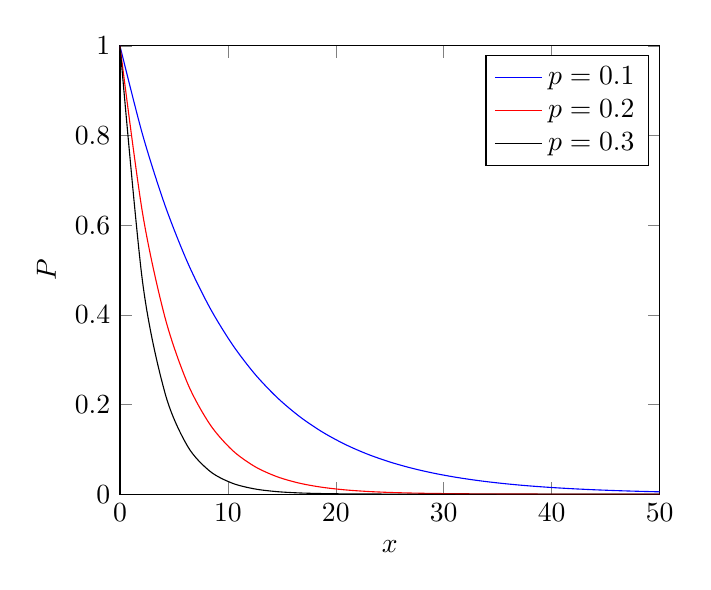
\begin{tikzpicture}
\begin{axis}[
    xlabel={$x$},
	ylabel={$P$},
	yticklabel style={/pgf/number format/fixed,
	    /pgf/number format/precision=1},
	xticklabel style={/pgf/number format/fixed,
	    /pgf/number format/precision=0},
	xmin = 0,
	xmax = 50,
	ymin = 0,
	ymax = 1.0,
	legend entries={$p=0.1$, $p=0.2$, $p=0.3$}
]
\addplot[blue,smooth,domain=0:50] { exp(x*ln(1-0.1) };
\addplot[red,smooth,domain=0:50] {exp(x*ln(1-0.2))};
\addplot[black,smooth,domain=0:50] { exp(x*ln(1-0.3) };
\end{axis}
\end{tikzpicture}
}
\bicaption[fig:procheck]{图索引}{成功骗过用户的概率和检测次数的关系}{Fig}{The relation between the possibility of succesful cheating and check times}
\end{figure}

我们的基于采样的验证是这样的:在系统的一般使用时为了效率考虑,用户都采用非验证搜索。然后随机的隔一段时间,用户在之前进行的搜索中随机抽出几个,用同样的关键词进行验证搜索。在收到验证搜索的结果后,用户先检验结果证明来保证这次验证搜索是正确的,然后用户在比对这次验证搜索的结果和之前同关键词的非验证搜索的结果。如果两次的结果一致,说明云服务在之前的那次非验证搜索时,没有欺骗用户,结果也是对的。

假设云服务商的搜索不是完全正确的,且错误情况是随机均匀分布的,其错误概率为p。比如说用户先是进行了n次非验证搜索。这时由于没有证明,用户是不知道云服务商给的结果是否是正确的。然后我们在这n非验证搜索中,随机抽查x个查询进行采样验证。那么这x个采样都通过,云服务成功骗过用户的概率为:$P = (1-p)^x$。

虽然从这个式子来看,云服务商成功骗过用户的概率和非验证搜索的次数n无关,但是考虑到云服务商可能会分析用户的采样规律,导致采样到云服务出错的情况降低,用户的非验证搜索次数还是要远大于采样数多比较好。

在图\ref{fig:procheck}中,我们列举了在几个不同的错误率上,云服务上成功骗过用户的概率和检测次数的关系。从图中,我们可以看出,云服务商成功骗过用户的概率是随采样次数呈指数级降低的。即使云服务上的错误率是在10\%,用户也只要进行50采样就能保证云服务商的错误不被发现的概率基本为0。

\subsection{和客户端验证的区别}
在第\ref{chap:relatedwork}章我们提到过一种客户端验证方式:用户在收到云服务商返回的查询结果后,从里面随机抽出几个查询,然后再本地重新进行搜索。最后通过对比本地搜索的结果和云服务商返回的结果来判断云服务商是否在欺骗用户。

通客户端验证方式类似,我们的基于采样的验证方式也是通过随机抽取一些查询来进行验证,也是只能在一定概率上保证正确性。但和客户端验证不同的是,我们的基于采样的验证方式,不需要用户在本地重新进行搜索,而只需要向云服务商提交一次或多次验证搜索。由于不需要在本地进行搜索,用户不仅节约了很多本地计算时间,还不需要在本地保存文档和索引这些非常占用空间的数据。由于不需要在本地保存文档和索引数据,用户就可以方便的在不同的客户端比如PC、平板或手机上进行查询和采样验证。

我们的采样验证方式之所以比客户端验证方式多了这些优点,是因为我们的系统可以在云服务商生成结果证明。而对于一般的客户端验证方式,云服务上没有这个功能,就只能要用户在本地重新搜索来验证结果的正确性。

%\section{系统展示}
\section{本章小结}
本章介绍了我们的云计算快速验证系统的设计与实现。为了系统的易维护性和可扩展性,我们采用了分节点的设计,每个节点为单独的进程,各个节点之间使用HTTP协议交互,这样不同的节点可以部署到不同的机器,也使得我们的系统可以方便地部署到多台机器机器。
由于对于一些搜索结果文档数目巨大的关键词,正确性证明的计算相当缓慢,这直接影响了整个系统的效率。
为了加快证明的生成,我们设计了树状结构的证明,将一个大的集合拆分成多个小的集合,是的正确性证明的计算不需要用的整个集合的元素,减少了计算量。同时各个小集合的计算可以多机器多进程并行计算,使得效率进一步提高。
在我们的实现中,我们设计了一套轻量级的并行计算框架来计算树状结构结构。通过使用这套并行计算框架,我们可以根据数据量的大小,选择合适数目的机器来进行计算。
在使用树状结构证明优化了正确性证明的生成之后,我们还设计了一个将完整性证明也用Membership Witness表示的方法,使树状结构也可以用于完整性证明的生成上。
我们还考虑了一种效率优先而正确性保证可以降低的情况。对于这种情况,我们提出了一种基于采样的验证方式。在这种方式下,用户平时使用的是不需要结果证明的搜索。然后用户在随机的时间,随机选取之前进行过的搜索让云服务商进行带结果证明的搜索。用户可以比较两次搜索的结果来判断云服务商是否有出错的情况。这种基于采样的验证方式使得用户可以在搜索效率和正确性保证度之间进行选择,选择一个适合自己的权衡。
